\documentclass{article}
\usepackage[utf8]{inputenc}
\usepackage[margin = 0.8in]{geometry}
\usepackage{graphicx}
\usepackage{amsmath, amssymb}
\usepackage{subcaption}
\usepackage{multirow}
\usepackage{mathtools}
\usepackage{float}


\title{RBE502 - Homework Set 9}
\author{Keith Chester}
\date{Due date: November 3 2021}

\begin{document}
\maketitle

\section*{Introduction}
In this assignment, we are charged with exploring various path planning algorithms - specifcally depth-first-search (DFS), breadth-first-search (BFS), and Dijkstra's search. We also explore A* and greedy bst-first search (greedy) search, and completey random neighbor selection (random) algorithms for comparison.

In this project, we are looking at a discrete space of a square grid. The grid consists of individual cells that are represented as occupied by an obstacle (a black square), as empty (a white square), the robot's starting position (a red square), and the goal (a green square). In our provided examples, an additional light blue square is used to show areas that were considered during path planning, but not utilized, and a dark blue square for the final generated path. For movement, we only consider orthogonal movement, no diagonals.

\section*{How Each Planner Works}
For our initial planners, BFS and DFS, we operate exactly the same but store our considered neighbors into different queues. For BFS, we utilize a FIFO (first in, first out) queue to explore the breadth of each neighbor before diving a level deeper. For DFS, we utilize a LIFO (last in, first out) queue to explore the depth of possible children before considering breadth of other adjacent neighbors.

For our random planner, we simply store all neighbors in a list and choose from our queue randomly each time we consider a new node.

For our remaining planners, we use priority queues with slightly different scoring techniques. Defining a $g(x)$ as a cost function for moving to each cell, we increment the cost to reach each cell by one for each cell we've moved from the start. When we encounter a cell that we have encountered prior as a possible new neighbor, we check to see if we have a lower cost to reaching this neighbor than before; if so, we note the new cost and mark the node as having a new "parent" for once a path is found. For Dijkstra's, the cost $g(x)$ is utilized alone.

We then introduce a heuristic function $h(x)$ - which, for our example, is a simple Euclidean distance function bewteen $g$ goal and $c$ current $d = \sqrt{(x_g - x_c)^2 - (y_g - y_c)^2}$. For our greedy function, we use the priority queue with this alone defining the priority of each cell. For A*, we utilize a priority defined by $g(x) + h(x)$ - or, the cost to reach each cell with the estimated distance to the goal. Cells that are easier to reach that are closer to the goal are thus prioritized.

\section*{Examples}
Here we see a an example map of 128x128 grid cells. In this example, we fill the map with obstacles until we hit a desired coverage percentage - in this case, $ 35\% $ coverage. We see the total considered cells and final path from the robot's starting position to its goal.

\begin{figure}[H]
    \centering
    \begin{subfigure}{0.45\textwidth}
        \centering
        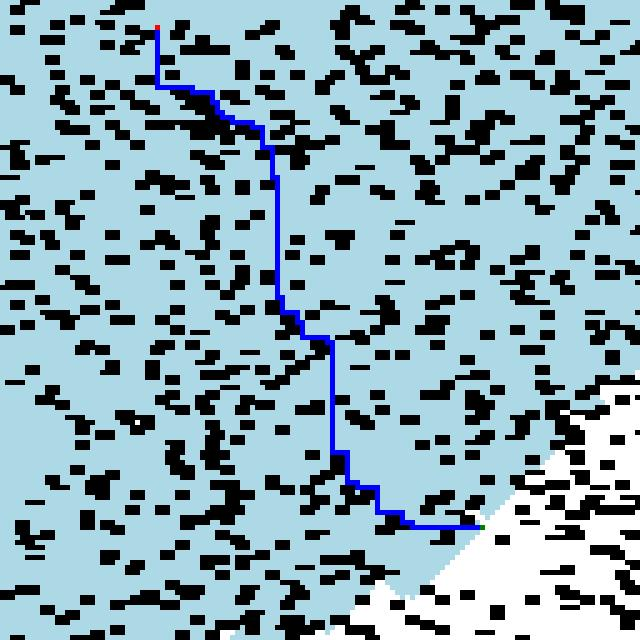
\includegraphics[width = \textwidth]{images/bfs.jpg}
        \caption{Breadth first search (BFS)}
    \end{subfigure}
    \begin{subfigure}{0.45\textwidth}
        \centering
        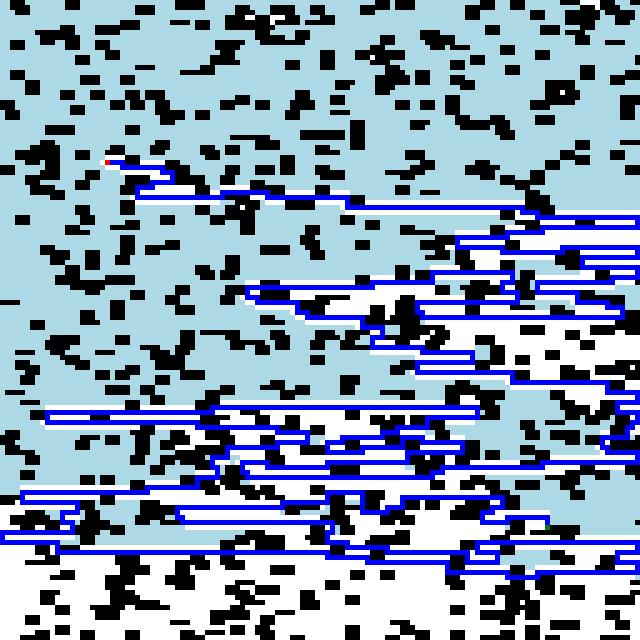
\includegraphics[width = \textwidth]{images/dfs.jpg}
        \caption{Depth first search (DFS)}
    \end{subfigure}
    \begin{subfigure}{0.45\textwidth}
        \centering
        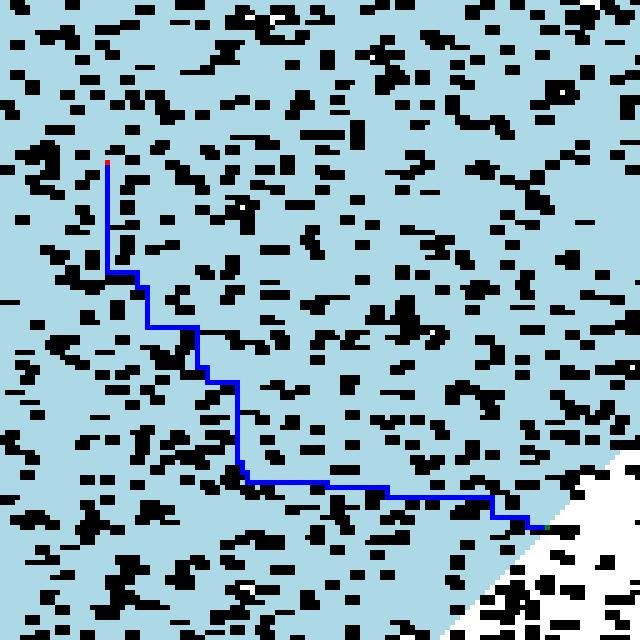
\includegraphics[width = \textwidth]{images/dijkstras.jpg}
        \caption{Dijkstras}
    \end{subfigure}
    \begin{subfigure}{0.45\textwidth}
        \centering
        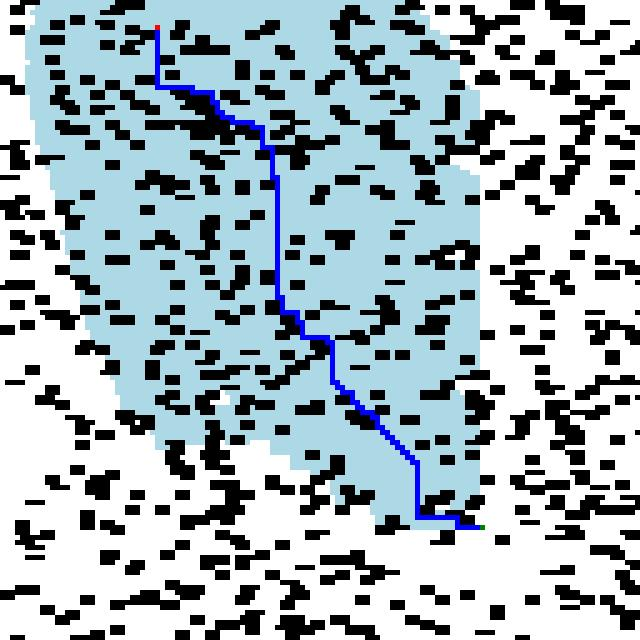
\includegraphics[width = \textwidth]{images/astar.jpg}
        \caption{A*}
    \end{subfigure}
    \begin{subfigure}{0.45\textwidth}
        \centering
        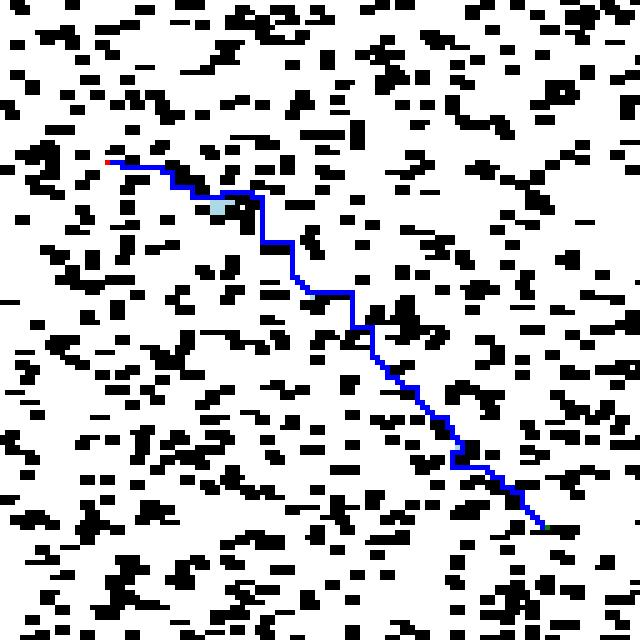
\includegraphics[width = \textwidth]{images/greedy.jpg}
        \caption{Greedy}
    \end{subfigure}
    \begin{subfigure}{0.45\textwidth}
        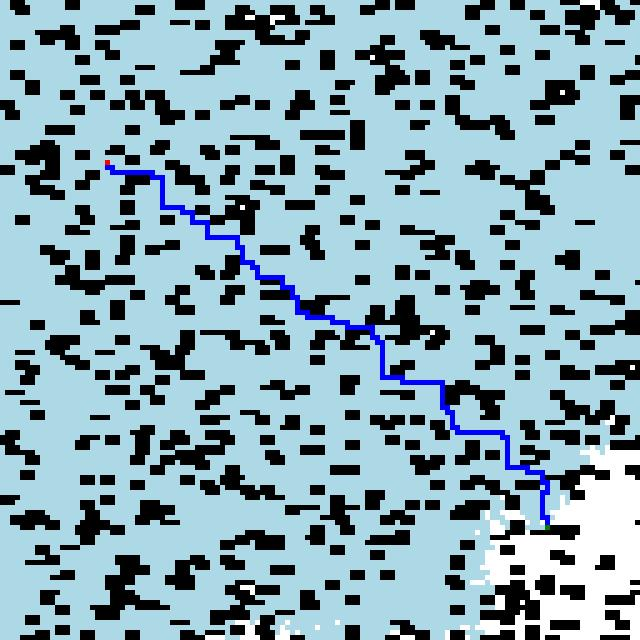
\includegraphics[width = \textwidth]{images/random.jpg}
        \caption{Random}
    \end{subfigure}
    \caption{Example maps with solved paths for each algorithm}
    \label{fig:example-maps}
\end{figure}

In our above figure of example maps, light blue cells emitting outward from the start (red) until it reaches the goal (green), and a dark blue path to the goal. For BFS we see the majority of the map covered, and then the optimal path towards the goal. DFS is far crazier - since the algorithm continually digs deeper into the children of each neighbor before electing to explore another, earlier child, we see a wild exploration before we see an equally wild and inefficient route. Dijkstras matches the BFS image, which we discuss later in the \textbf{Results and Conclusions} section. For our A* search, we see a similar outward branching that we see in BFS and Dijkstras, but to a lesser extreme due to its use of a heuristic function (in our case, Euclidean distance to the goal from current position). The optimal path is still found. Our greedy search - which only looks at the heuristic of distance to goal and not at all the to-reach cost that Dijkstra's and A* would, seems to explore less space but finds a non optimal route to the goal. Finally, for our random search,it appears to be just that - random until 

\section*{Performance}

We took each algorithm and plot total iterations taken to find a solution and the resulting path length, as well as all algorithms overlayed. We explored each algorithm from $0\%$ obsacle coverage to $75\%$ coverage with increments of $5\%$. For each algorithm and percentage combination, we randomly generate 500 solvable maps and perform the solution. If a generated map was not solvable (no path existed), we would ignore that attempt for our total of 500.

The individual performance of each algorithm is shown below:

\begin{figure}[H]
    \centering
    \begin{subfigure}{0.325\textwidth}
        \centering
        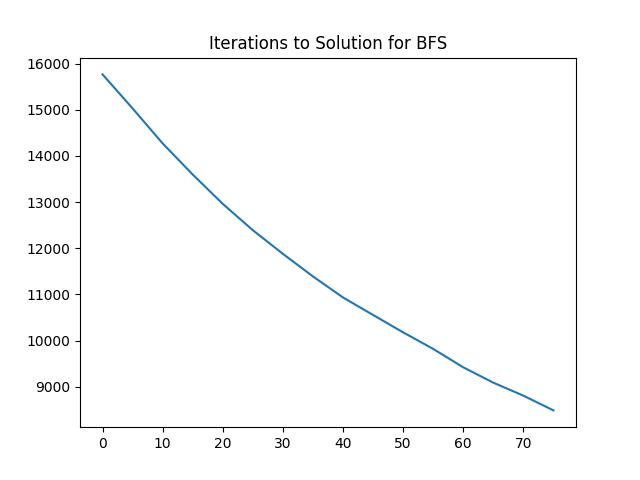
\includegraphics[width = \textwidth]{plots/BFS_iterations.jpg}
        \caption{Breadth first search (BFS)}
    \end{subfigure}
    \begin{subfigure}{0.325\textwidth}
        \centering
        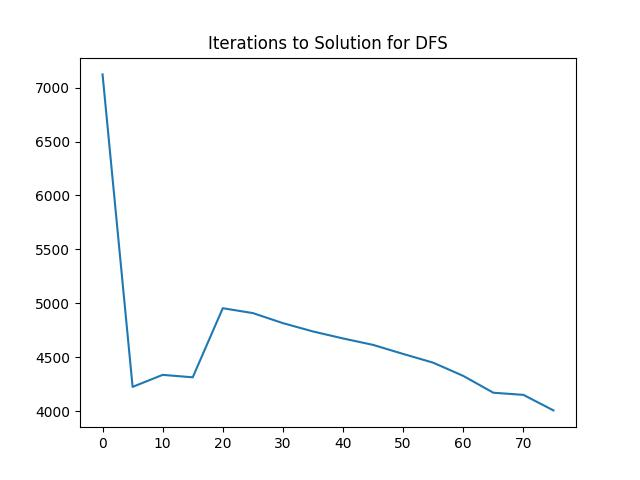
\includegraphics[width = \textwidth]{plots/DFS_iterations.jpg}
        \caption{Depth first search (DFS)}
    \end{subfigure}
    \begin{subfigure}{0.325\textwidth}
        \centering
        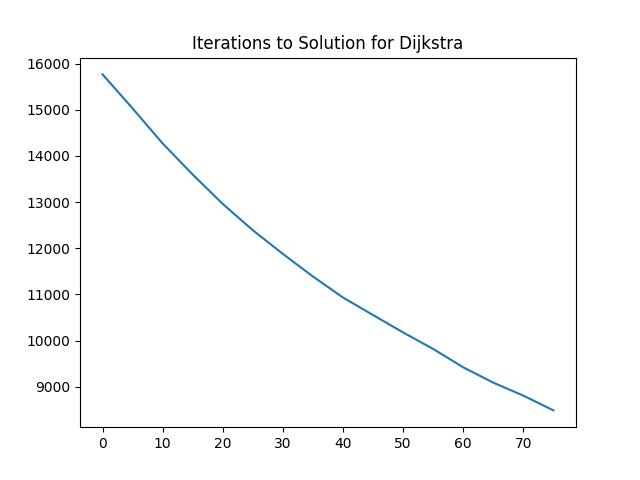
\includegraphics[width = \textwidth]{plots/Dijkstra_iterations.jpg}
        \caption{Dijkstras}
    \end{subfigure}
    \begin{subfigure}{0.325\textwidth}
        \centering
        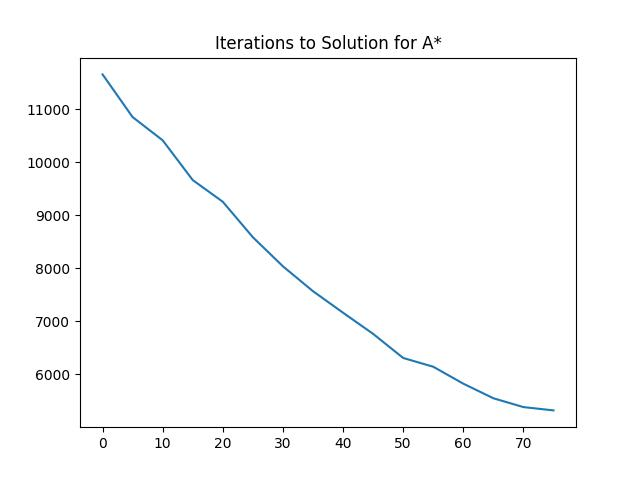
\includegraphics[width = \textwidth]{plots/A*_iterations.jpg}
        \caption{A*}
    \end{subfigure}
    \begin{subfigure}{0.325\textwidth}
        \centering
        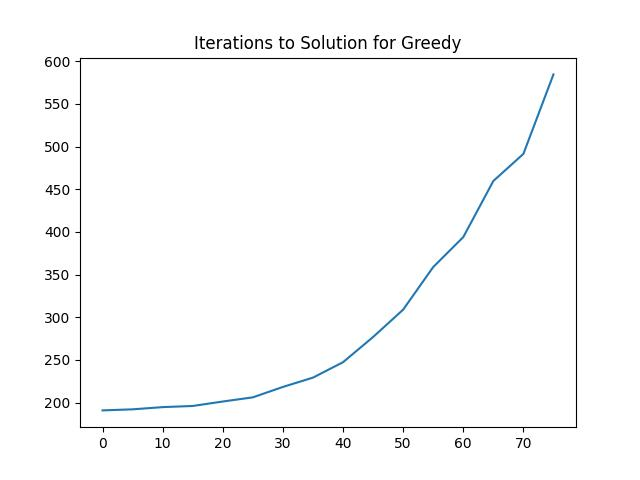
\includegraphics[width = \textwidth]{plots/Greedy_iterations.jpg}
        \caption{Greedy}
    \end{subfigure}
    \begin{subfigure}{0.325\textwidth}
        \centering
        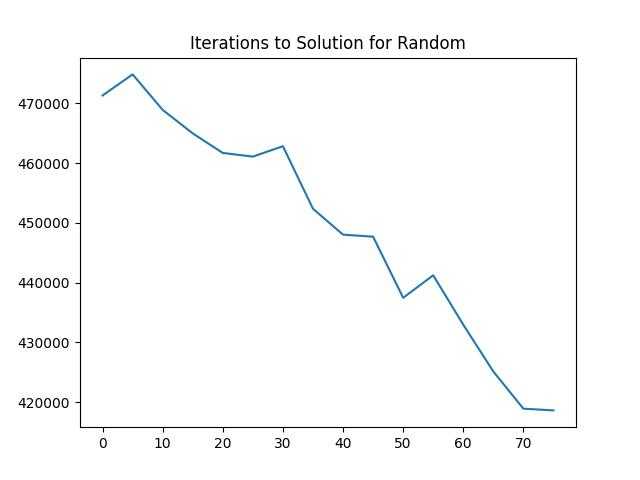
\includegraphics[width = \textwidth]{plots/Random_iterations.jpg}
        \caption{Random}
    \end{subfigure}
    \caption{Iterations per planner algorithm}
    \label{fig:iterations-per-planner}
\end{figure}

\begin{figure}[H]
    \centering
    \begin{subfigure}{0.325\textwidth}
        \centering
        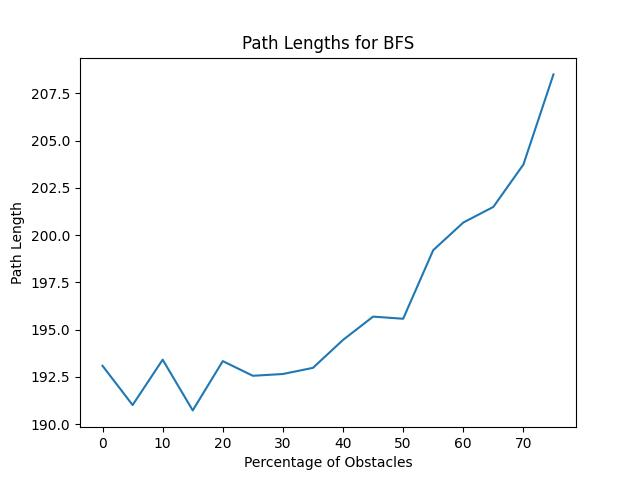
\includegraphics[width = \textwidth]{plots/BFS_paths.jpg}
        \caption{Breadth first search (BFS)}
    \end{subfigure}
    \begin{subfigure}{0.325\textwidth}
        \centering
        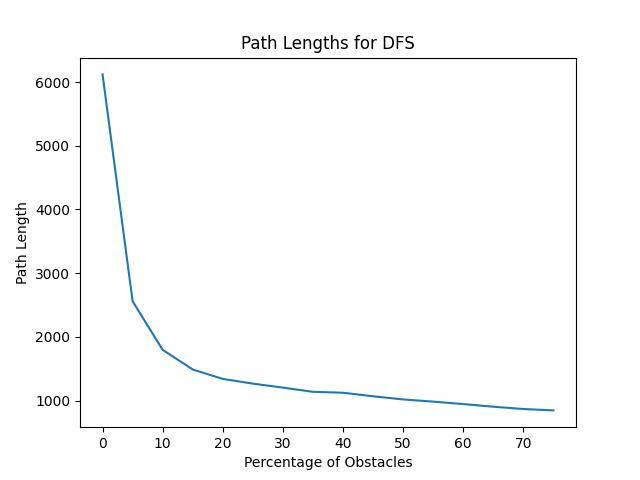
\includegraphics[width = \textwidth]{plots/DFS_paths.jpg}
        \caption{Depth first search (DFS)}
    \end{subfigure}
    \begin{subfigure}{0.325\textwidth}
        \centering
        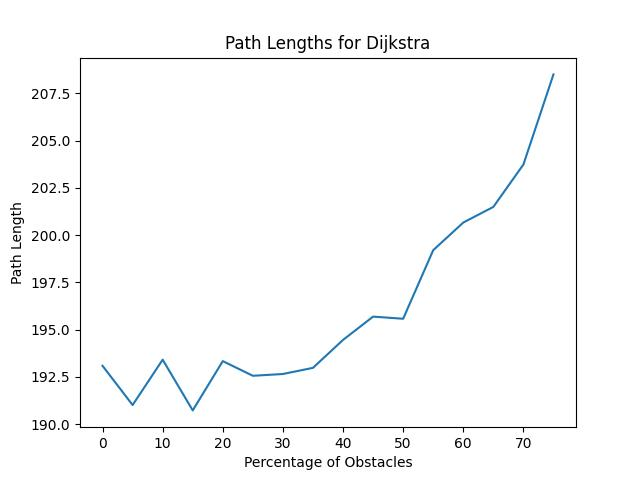
\includegraphics[width = \textwidth]{plots/Dijkstra_paths.jpg}
        \caption{Dijkstras}
    \end{subfigure}
    \begin{subfigure}{0.325\textwidth}
        \centering
        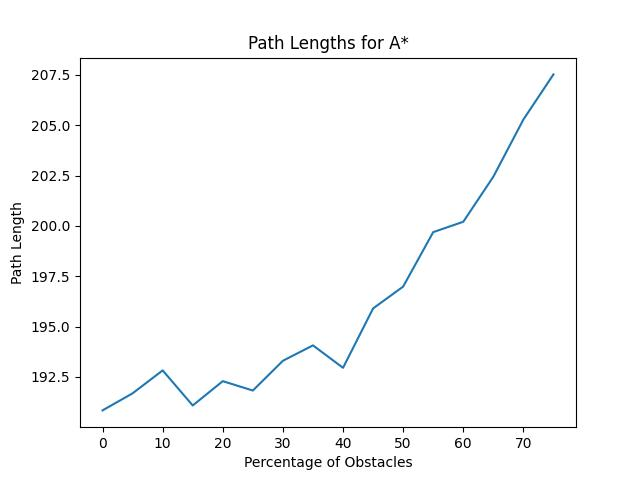
\includegraphics[width = \textwidth]{plots/A*_paths.jpg}
        \caption{A*}
    \end{subfigure}
    \begin{subfigure}{0.325\textwidth}
        \centering
        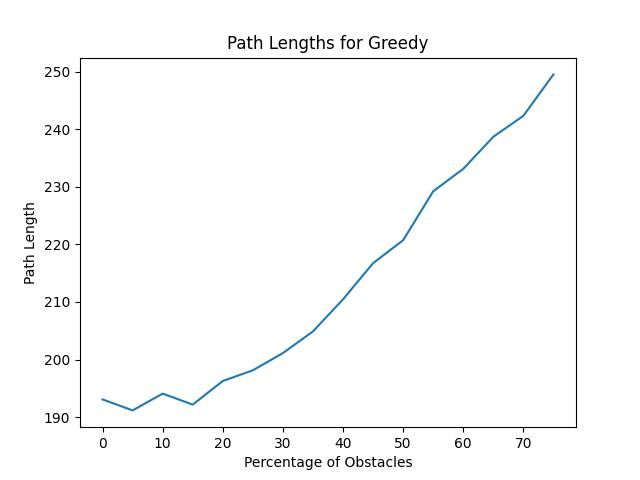
\includegraphics[width = \textwidth]{plots/Greedy_paths.jpg}
        \caption{Greedy}
    \end{subfigure}
    \begin{subfigure}{0.325\textwidth}
        \centering
        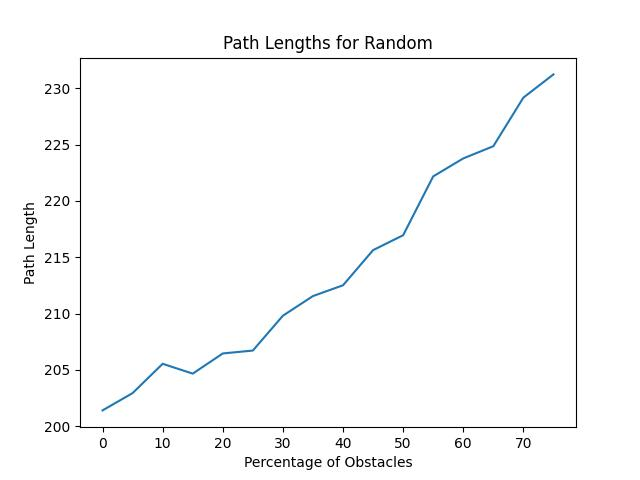
\includegraphics[width = \textwidth]{plots/Random_paths.jpg}
        \caption{Random}
    \end{subfigure}
    \caption{Path length averag per each planner algorithm}
    \label{fig:paths-per-planner}
\end{figure}

Finally, we overlay the data for planner for comparison:

\begin{figure}[H]
    \centering
    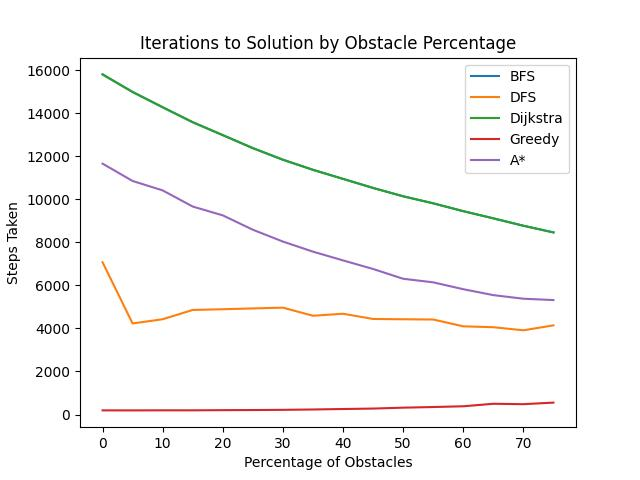
\includegraphics[width = 0.75\textwidth]{plots/steps_taken.jpg}
    \caption{Iterations for each planner algorithm overlayed}
    \label{fig:iterations-all}
\end{figure}

\begin{figure}[H]
    \centering
    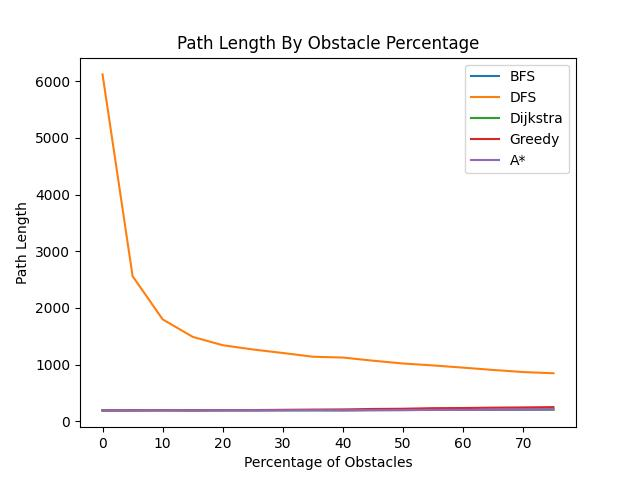
\includegraphics[width = 0.75\textwidth]{plots/path_length.jpg}
    \caption{Iterations per planner algorithm}
    \label{fig:paths-all}
\end{figure}

...and since DFS creates such inefficient routes, we look at that last chart again with DFS removed:

\begin{figure}[H]
    \centering
    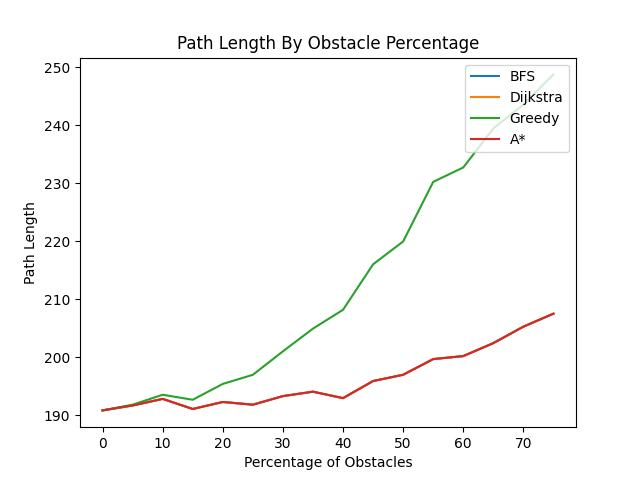
\includegraphics[width = 0.75\textwidth]{plots/path_length_sans_dfs.jpg}
    \caption{Iterations per planner algorithm, sans DFS}
    \label{fig:paths-sans-dfs}
\end{figure}

In these figures we see on our overlayed algorithms several algorithms overlap, resulting in some algorithms appearing as if they are missing. This is explained in our below section.

\section*{Results and Conclsuions}

In this assignment, it appearsa the BFS and Dijkstras perform the same, but we know their applications are different. Why is this? Note that our grid represents a discrete space with equal cost between all neighboring cells - which in our algorithms would be displayed as an unweighted graph. For an unweighted graph, BFS and Dijkstra's algorithm perform identically. If the graph was weighted, ie varying costs between neighboring cells driven by some rule-set, Dijkstra's would have less iteratons to find the optimal solution than BFS.

BFS, Dijkstra's, and A* all find the optimal path, though A* is dependent upon an admissible heuristic function. With the simplicity of our example we utilized Euclidean distance to the node for our heuristic.

DFS as an algorithm creates wildly inefficient routes, but can quickly discover if a path exists. However, it does find routes with at a fairly steady rate irregardless of obstacle prolificness. Our greedy algorithm, however, which has a queue that prioritizes entirely off a heuristic of Euclidean distance to the goal, proved to be even quicker a path to the goal. The greedy approach does not gaurantee the optimal route that BFS, Dijkstra's, or A* does, but performs similarly until obstacle percentage raises.

In all, if the graph is unweighted, there is no discernable difference between BFS and Dijkstra's, and a noticeable improvement with A*. If the graph is weighted, A* would still be the preferred choice. If we were aiming to find if any path to the goal exists as quickly as possible, and we are confident in a low probability of obstacles between us and the path, we may find use in utilizing the greedy approach for a more rapid check.optimal path, however.


\end{document}